\documentclass[letterpaper]{article}
\usepackage{aaai}
\setlength{\textwidth}{5in}
\setlength{\oddsidemargin}{.75in}
\setlength{\evensidemargin}{.75in}
\usepackage{palatino}
\usepackage[utf8]{inputenc}
\usepackage{helvet}
\usepackage{amsmath, amsfonts, amssymb, amsthm}
%\usepackage{graphicx}
\usepackage[center]{caption}
\usepackage{subcaption}
%\usepackage{epstopdf}
\usepackage{multirow}
%\usepackage{color}
%\graphicspath{{./figures/}}
\usepackage{courier}
\usepackage{tabularx}
\usepackage{endnotes}
\usepackage{booktabs}
\usepackage{url}
\usepackage{wrapfig}
\makeatletter
\def\url@leostyle{%
  \@ifundefined{selectfont}{\def\UrlFont{\sf}}{\def\UrlFont{\rmfamily}}}
\makeatother
\urlstyle{leo}
\usepackage{fixltx2e}
\usepackage[none]{hyphenat}
\usepackage{microtype}
\DisableLigatures{encoding = *, family = *}
\frenchspacing
\raggedright
\setlength{\parindent}{10pt}
\let\footnote=\endnote
\title{Capturing Planned Protests from Open Source Indicators}
\author{Sathappan Muthiah, Bert Huang, Jaime Arredondo,\\
{\bf \large David Mares, Lise Getoor, Graham Katz and Naren Ramakrishnan}}
\nocopyright

\begin{document}
\newcommand{\then}{\Rightarrow}
\newcommand{\softor}{\operatornamewithlimits{{\vee}}}
\newcommand{\softand}{\operatornamewithlimits{{\wedge}}}
\newcommand{\softthen}{\operatornamewithlimits{{\then}}}
\newcommand{\softneg}{\operatornamewithlimits{{\neg}}}

%\theoremstyle{plain}
\newtheorem{exmp}{Example}
\maketitle
\onecolumn

%Don't be alarmed because the abstract begins on a new page. That is intentional. Your final article won't look like this.

\begin{quote} %Don't put a heading on your abstract.
Civil unrest events (protests, strikes, and ``occupy'' events) are common
occurrences in both democracies and authoritarian regimes. The study of civil
unrest is a key topic for political scientists as it helps capture an important
mechanism by which citizenry express themselves. In countries where civil
unrest is lawful, qualitative analysis has revealed that more than 75\% of the
protests are planned, organized, and/or announced in advance; therefore
detecting references to future planned events in relevant news and social media
is a direct way to develop a protest forecasting system. We report on a system
for doing that in this paper. It uses a combination of keyphrase learning to
identify what to look for, probabilistic soft logic to reason about location
occurrences in extracted results, and time normalization to resolve future time
mentions. We illustrate the application of our system to 10 countries in Latin
America, viz. Argentina, Brazil, Chile, Colombia, Ecuador, El Salvador, Mexico,
Paraguay, Uruguay, and Venezuela. Results demonstrate our successes in
capturing significant societal unrest in these countries with an average lead
time of 4.08 days. We also study the selective superiorities of news media
versus social media (Twitter, Facebook) to identify relevant trade-offs.
\end{quote}

%############INTRODUCTION##################################

Civil unrest events (protests, strikes, and ``occupy'' events) are
common occurrences in both democracies and in authoritarian regimes.
Although we typically associate civil unrest with disruptions and
instability, social scientists believe that civil unrest reflects the
democratic process by which citizenry communicate their views and
preferences to those in authority.  The advent of social media has
afforded citizenry new mechanisms for organization and mobilization, and
online news sources and social networking sites like Facebook and
Twitter can provide a window into civil unrest happenings in a
particular country.

%\begin{figure*}
\begin{wrapfigure}{r}{.4\textwidth}
  \centering
    %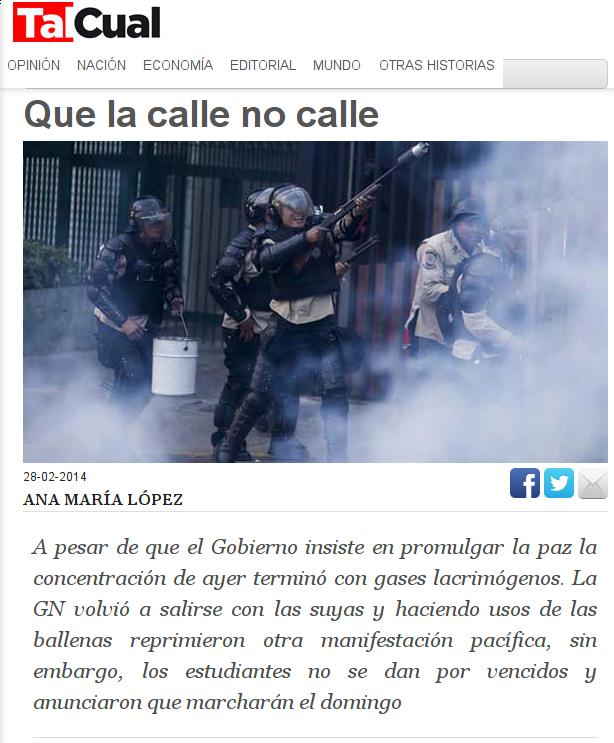
\includegraphics[width=.4\textwidth]{pp_AIMag_screenshot}
    \caption{An example article describing plans for a future protest (Venezuela, June 11, 2014).}
    \label{pp_example}
\end{wrapfigure}
%\end{figure*}

\subsubsection{Why study and forecast protests?}
Our primary region of interest is Latin America (secondary regions of
interest include the Middle East and North Africa), and protest is an
important topic of study in this region, as many countries here are
democracies struggling to consolidate themselves. The combination of
weak channels of communication between citizen and government, and a
citizenry that still has not grasped the desirability of elections as
the means to affect politics means that public protest will be an
especially attractive option. To illustrate the power of protest in
Latin America we need only recall that between 1985 and 2011, 17
presidents resigned or were impeached under pressure from
demonstrations, usually violent, in the streets. Protests have also
resulted in the rollback of price increases for public services, such as
during the Brazilian Spring of June 2013.

Forecasting protests is an important capability in many domains.  For
the tourism industry, forecasting protests can support the issuance of
travel warnings. For law enforcement, forecasting protests can aid in
preparedness. For social scientists, forecasting protests will provide
insight into how citizens express themselves.  For governments, a
protest forecasting system can help prioritize citizen grievances.
Finally, protests can have a debilitating effect on multiple industries
(especially those that rely on worldwide supply chain management) and
thus a protest forecasting system can aid in planning and design of
alternative travel and shipping routes.

\subsubsection{Planned protests}
Our basic hypothesis is that protests that are larger will be more
disruptive and communicate support for its cause better than smaller
protests.  Mobilizing large numbers of people is more likely to occur if
a protest is organized and the time and place announced in advance.
Because protest is costly and more likely to succeed if it is large, we
should expect planned, rather than spontaneous, protests to be the norm.
Indeed, in a sample of 288 events from our study selected for
qualitative review of their antecedents, for 225 we located
communications regarding the upcoming occurrence of the event in media,
and only 49 could be classified as spontaneous (we could not determine
whether communications had or had not occurred in the remaining 14
cases).

\subsubsection{EMBERS (Early Model Based Event Recognition using
Surrogates)}
We are an industry-university partnership charged with developing an
automatic protest forecasting system for 10 countries in Latin America
(LA) and 7 countries in the Middle East and North Africa region (MENA).
Our system, called EMBERS, has been deployed since Nov 2012 and has been
generating forecasts (called warnings or alerts) automatically, without
a human-in-the-loop, since then (the MENA region was added in July
2014). These forecasts are emailed to a third party (MITRE) for
evaluation. Analysts at MITRE organize a reference database of protests
(called the Gold Standard Report, or GSR) by surveying newspapers for
reports of protests, and compare our warnings against the GSR to
generate a scoring report, using evaluation criteria described later.

The full EMBERS system has been described elsewhere~\cite{emberskdd,DBLP:conf/bigdataconf/DoyleKSAZLMZLBKFR14}, including
the overall system architecture, data sources used for analysis, and the
various forecasting models that make up the system. EMBERS adopts a multi-model approach,
wherein different models are leveraged for their selective superiorities
to generate a fused set of alerts. One of the
best performing models in EMBERS is the planned protest model that detects
ongoing organizational activity and generates warnings accordingly. This paper
is the first to present this model in detail, including the 
research issues involved, and how we addressed them in EMBERS.

Capturing mentions of protest planning and organization is not as easy
as it might appear. First, articles of interest are written in different
languages (Spanish, Portuguese, French, Dutch, and English).  Second,
multiple locations are often mentioned in a given article, leading to
(natural language) ambiguity about the intended location of the event.
Significant reasoning is required to discern the correct protest
location.  Finally, identifying the date of a planned event in Latin
America involves significant multilingual temporal-semantic natural
language processing as dates are often described with vague, relative,
or otherwise context-dependent expressions (e.g., {\em Sunday} or {\em
in two days}).


Our detection approach combines shallow linguistic analysis to identify
relevant documents (articles, tweets) with targeted deep semantic
analysis of the selected documents. Despite its simplicity, this
approach is capable of detecting indicators of event planning with
surprisingly high accuracy.

Our contributions are:

\begin{enumerate}
\item We present a protest forecasting system that couples three key
  technical ideas: keyphrase learning to identify what to look for,
  probabilistic soft logic to reason about location occurrences in
  extracted results, and date normalization to resolve future tense
  mentions. We demonstrate how the integration of these ideas achieves
  objectives in precision, recall, and quality (accuracy).
\item We illustrate the application of our system to 10 countries in
  Latin America, viz. Argentina, Brazil, Chile, Colombia, Ecuador, El
  Salvador, Mexico, Paraguay, Uruguay, and Venezuela. Our system
  predicts the {\it when} of the protest as well as {\it where} of the
  protest (down to a city level granularity).  We conduct ablation
  studies to identify the relative contributions of news media (news +
  blogs) versus social media (Twitter, Facebook) to identify future
  happenings of civil unrest. Through these studies we illustrate the
  selective superiorities of different sources for specific countries.
\item Unlike many studies of retrospective forecasting of protests, our
  system has been {\bf deployed and in operation for nearly three
  years.} The end consumers of our alerts are analysts studying Latin
  America.
Our results demonstrate that we are able to capture significant societal
unrest in the above countries with an average lead time of 4.08 days. 
\end{enumerate}

%###################RELATED WORK ##################################
\section{Related Work}
Five categories of related work are briefly discussed here (see also
Table~\ref{comp-table}).

{\bf Event detection via text extractions}
is an extensively studied topic in the literature. Document clustering techniques are used 
in, e.g.,~\cite{Gabrilovich:2004:NPP} to identify events retrospectively or as the stories arrive.
Works like~\cite{Banko07openinformation,Chambers:2011:TIE,riloff2003learning} focus on
extraction patterns (templates) to extract information from text. 

{\bf Temporal information extraction} is another well studied topic.
The TempEval challenge~\cite{tempeval} led to a significant amount of
algorithmic development for temporal NLP.
For instance a specification language
for temporal and event expressions in natural language text is described in~\cite{timeml}.
References~\cite{LlorensDGS12} and~\cite{tempex} provide methods to
resolve temporal expressions in text (our own work here uses the TIMEN
package~\cite{LlorensDGS12} and more recently the HeidelTime
package~\cite{strotgen2014time}).

{\bf Event forecasting:} 
Radinsky and Horvitz~\shortcite{Radinsky:2013:MWP} find event sequences
from a corpora and then use these sequences to determine if an event of
interest (e.g., a disease outbreak, or a riot) will occur sometime in
the future. This work predicts only if a potential event will happen
given a historical event sequence but does not geolocate the event to a
city-level resolution, as we do here.  Kallus~\shortcite{nathankallus}
make use of event data from RecordedFuture~\cite{recordedFuture} to
determine if a  significant protest event will occur in the subsequent
three days and casts this as a classification problem.  This work only
focuses on prediction of significant events (suitably defined) and the
forecast is limited to a fixed time window of the next three days. 

{\bf Future retrieval:}
Baeza-Yates~\shortcite{baeza2005searching} provides one of the earliest
discussions of this topic; here future temporal information in text is
found and used to retrieve content from search queries that combine both
text and time with a simple ranking scheme.  Kawai et
al.~\shortcite{Kawai:2010:CSE} present a search engine (ChronoSeeker)
for searching future and past events.
RecordedFuture~\cite{recordedFuture}, introduced earlier, conducts
real-time analysis of news and tweets to identify mentions of events
along with associated times. Anecdotally it is estimated that
approximately (only) 5--7\% of events extracted by RecordedFuture are
about the future.

{\bf Planned protest detection:}
Two publications---Compton et al.~\shortcite{compton2013detecting} and
Xu et al.~\shortcite{xu2014civil}---align very closely to our own work
as their emphasis is on protest forecasting.  Both works are aimed at
forecasting protests but emphasize different data sources and different
methodologies. For instance, the work in~\cite{compton2013detecting}
filters the Twitter stream for keywords of interest and searches for
future date mentions in only absolute terms, i.e., explicit mentions of
a month name and a number (date) less than 31.  Such an approach will
not be capable of extracting the more common way in which future dates
are referenced, e.g., phrases like ``tomorrow,'' ``next tuesday.'' The
work in~\cite{xu2014civil} by the same group of authors uses the Tumblr
feed with a smaller set of keywords but again is restricted to the use
of absolute time identifiers.

\newpage
\begin{table}
    \centering
    \footnotesize
    \caption{Comparison of our approach against other techniques.}
    \begin{tabularx}{\textwidth}{p{5cm} XXXX}%{|*{17}{c|}}
        \toprule
        & Relative date resolution & Ingest multiple sources? & Reasoning about location & Learning word/phrase filters \\
        \midrule
        `Future' Search Engines~\cite{Kawai:2010:CSE,Jatowt:2011:ECE,baeza2005searching}&\checkmark & & \\
        Time-to-Event Recognition~\cite{tops2013predicting,bosch2013estm}&\checkmark & & \\
        Planned Protest Detection~\cite{xu2014civil,compton2013detecting} & &\checkmark & &\\ 
        This paper &\checkmark &\checkmark &\checkmark&\checkmark\\
        \bottomrule
    \end{tabularx}
\label{comp-table}
\end{table}
\newpage
~
\newpage

%#####################PSL####################################
\section{Probabilistic Soft Logic}
  \label{section:PSL}
In this section, we briefly describe probabilistic soft logic
(PSL)~\cite{kimmig2012short}, a key component of our geocoding strategy.
PSL is a framework for collective probabilistic reasoning on relational
domains.  PSL represents the domain of interest as logical atoms.  It
uses first order logic rules to capture the dependency structure of the
domain, based on which it builds a joint probabilistic model over all
atoms.  Instead of hard truth values of \textrm{0} (false) and
\textrm{1} (true), PSL
uses soft truth values relaxing the truth values to the interval
\textrm{[0,1]}.  The logical connectives are adapted accordingly.

User defined \emph{predicates} are used to encode the relationships and
attributes and \emph{rules} capture the  dependencies and constraints.
The rules can also be labeled with non-negative weights which are used
during the inference process.  The set of predicates and weighted rules
thus make up a PSL program where known truth values of ground atoms
 are derived from observed data and unknown truth values for the remaining
atoms are learned using the PSL inference.

\begin{exmp}
We will follow a running example throughout this section. In our
geocoding subtask, we create a PSL program that reasons about the
predicate \textsc{RefersTo}, which maps a text string to real-world
locations. For example, \textsc{RefersTo}(\textrm{``DC''},
\textrm{washingtonDC}) evaluates to true if the knowledge base believes
that  the article refers to Washington D.C.~as ``DC.'' This predicate gets
used in rules that define dependencies between predicates, such as the
rule
\begin{flalign*}
  \centering
  \textsc{Entity}&(L, \textrm{location}) \wedge \textsc{RefersTo}(L,\textrm{locID})
  \rightarrow \textsc{PSLLocation}(\textrm{Article}, \textrm{locID}), &
\end{flalign*}
which states that an entity extracted from an article text that matches
a known \textsc{RefersTo} mapping implies that the PSL program's
predicted location will follow that mapping. Some of these logical atoms
will be known as parts of a knowledge base, while others will be unknown
and will be inferred by PSL.
\end{exmp}

Given a set of atoms 
$\ell = \{\ell_1,\ldots,\ell_n\}$,
an interpretation defined as 
$I : \ell \rightarrow [0,1]^n$
is a mapping from atoms to soft truth values.  PSL defines a probability
distribution over all such interpretations such that those that satisfy
more ground rules are more probable.
\emph{Lukasiewicz t-norm} and its corresponding co-norm are used for
defining relaxations of the logical AND and OR respectively to determine
the degree to which a ground rule is satisfied.  Given an interpretation
\textit{I}, PSL defines the formulas for the relaxation of the logical
conjunction ($\wedge$), disjunction ($\vee$), and negation ($\neg$) as
follows:
\begin{align*}
\ell_1 \wedge \ell_2 &= \max\{0, I(\ell_1) + I(\ell_2) - 1\},\\
\ell_1 \vee \ell_2 &= \min\{I(\ell_1) + I(\ell_2), 1\},\\
\neg l_1 &= 1 - I(\ell_1),
\end{align*}  

The interpretation \textit{I} determines whether the rules are
satisfied. A rule $\mathit{r} \equiv \mathit{r_{body}} \rightarrow
\mathit{r_{head}} $  is satisfied if and only if the truth value of head
is at least that of the body. Otherwise, PSL uses a \emph{distance to
satisfaction}, which measures the degree to which this condition is
violated
\begin{center} 
 $\mathit{d_r}(\mathit{I}) =$ max\{0,$\mathit{I(r_{body})} - \mathit{I(r_{head})}$\}.
 \end{center}
 
\begin{exmp}
Continuing the previous example, if we have the rule
\begin{flalign*}
  \centering
  \textsc{Entity}&(\textrm{``Washington''}, \textrm{location}) ~ \wedge
  ~\textsc{RefersTo}(\textrm{``Washington''}, \textrm{washingtonDC}) &\\
  &\qquad \qquad\qquad \qquad \qquad ~~~~~~~\rightarrow
  \textsc{PSLLocation}(\textrm{Article},
  \textrm{washingtonDC}) &
\end{flalign*}
and the truth values of the known atoms are 
\begin{equation*}
  \begin{array}{rcl}
    \mbox{\textsc{Entity} (``Washington'', location)}                       & : & 1.0\\
    \mbox{\textsc{RefersTo}(\textrm{``Washington''},\textrm{washingtonDC})} & : & 0.6\\
  \end{array}
\end{equation*}
then following the relaxation of logical AND, the truth value of the
antecedent is $\max\{0, 1.0 + 0.6 - 1\} = 0.6$. Moreover, if the truth
value of the atom to be inferred, \textsc{PSLLocation}(\textrm{Article},
\textrm{washingtonDC}), is 0.1, then the distance to satisfaction of
this rule is $\max\{0, 0.6 - 0.1\} = 0.5$. On the other hand, if the
truth value of the head is 0.7, then the distance to satisfaction is
$\max\{0, 0.6 - 0.7\} = 0$, meaning the rule is satisfied.
\end{exmp}

PSL then induces a probability distribution over possible
interpretations \textit{I} over the given set of ground atoms
\textit{l} in the domain.  If \textit{R} is the set of all ground
rules that are instances of a rule from the system and uses only the
atoms in  \textit{I} then, the probability density function
\textit{f} over \textit{I} is defined as
\begin{equation}
\label{eq:contimn1}
    f (I) = \frac{1}{Z} \exp \left(-\sum_{r\in R} \lambda_r (d_r(I))^p \right)
\end{equation}
\begin{equation}
\label{eq:contimn2}
	Z = \int_{I} \exp \left( -\sum_{r\in R} \lambda_r (d_r(I))^p \right)
\end{equation}

where $\lambda_r$ is the weight of the rule \textit{r}, \textit{Z} is a normalization
constant, and $p \in {1, 2}$ provides a choice between linear or
quadratic loss functions, which produce different modeling behavior. PSL
further allows inclusion of linear equality and inequality constraints,
which enable modeling of functional constraints on the domains and
ranges of predicates. 

The probability distribution in Equation (1) is an example of a
\emph{hinge-loss Markov random field} \cite{bach:uai13}, which has a
form of energy function that makes inference of the most probable
explanation an efficient convex optimization. The expressiveness of PSL
and the efficiency of inference in its models allows us to encode
dependencies between various aspects of geolocation that are jointly
inferred.

\begin{exmp}
The joint probability distribution enables PSL to reason about
conflicting evidence, for example if we additionally have the atom
\mbox{\textsc{RefersTo}(``Washington'', Washington State)} in our
knowledge base with truth value 0.2, we would have two conflicting
\textsc{PSLLocation} implications.  The probabilistic, weighted rules,
as well as the soft truth values of known atoms control how much PSL
considers each piece of evidence, and additional corroborating or
conflicting evidence would also be incorporated into the final joint
inference.
\end{exmp}

%##################APPROACH ################
\section{Approach}
The general approach we adopt is to identify open-source documents that
appear to indicate civil unrest event planning, extract relevant
information from identified documents and use that as the basis for a
structured warning about the planned event. 
Each of these processing steps (see Fig.~\ref{flowchart}) is outlined
next.

\begin{figure*}
%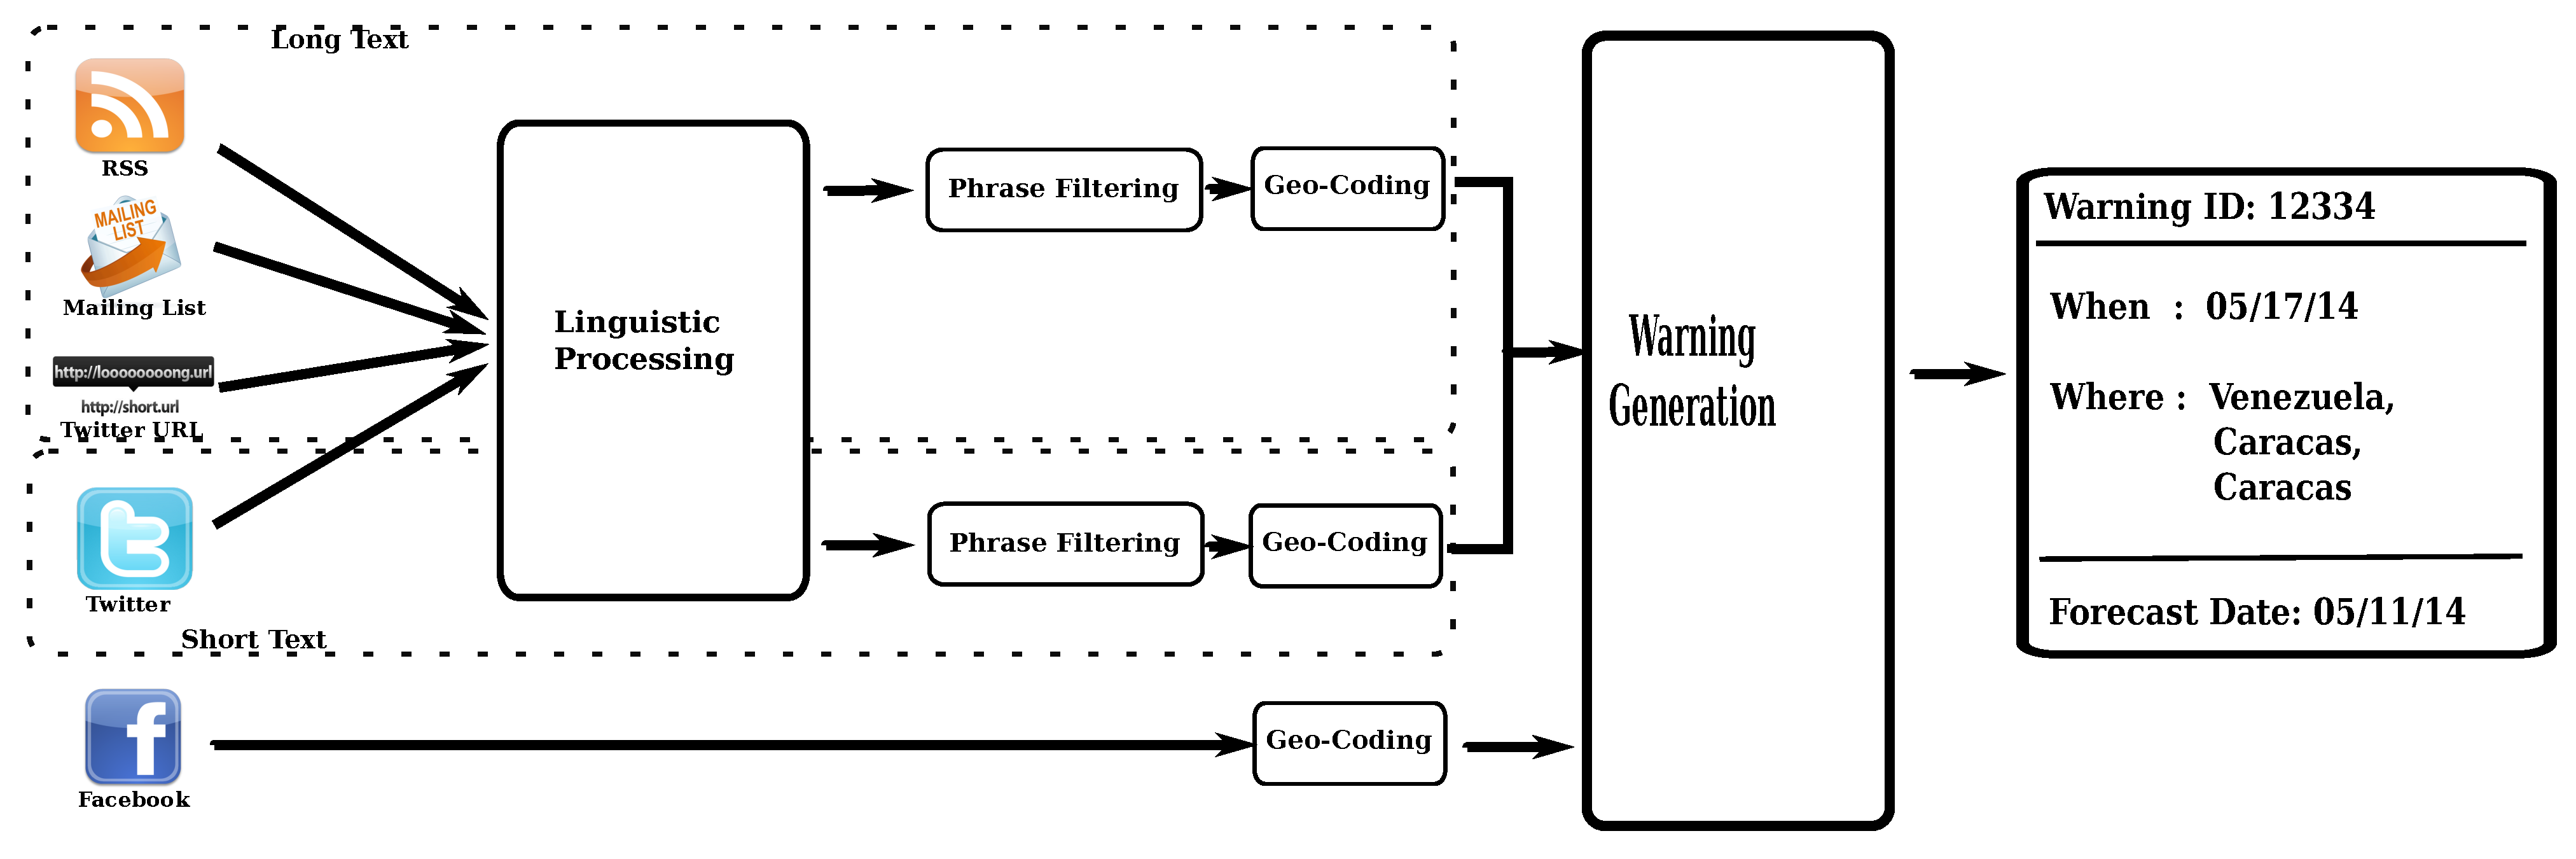
\includegraphics[width=\textwidth]{pipeline}
\caption{Schematic of the planned protest detector that ingests five
different types of data sources.}
\label{flowchart}
\end{figure*}

\subsection{Linguistic Preprocessing}
Since our region of interest is Latin America as well as the Middle East
and North Africa, the collection of text harvested is inherently
multilingual, with Spanish, Portuguese, Arabic, and English as the
dominating languages. Ingested documents are subjected to shallow
linguistic processing prior to analysis.  This initial processing
involves identifying the language of the document, distinguishing the
words (tokenization), normalizing words for inflection (lemmatization),
and identifying expressions referring to people, places, dates and other
entities.  We use Basis Technology's Rosette Linguistics Platform (RLP)
suite of multilingual commercial tools
(\url{http://www.basistech.com/text-analytics/rosette/}) for this
processing.  The output of this linguistic preprocessing serves as input
to subsequent deeper analysis in which date expressions are normalized,
sentences that appear to be describing protest planning are identified,
and the geographic focus of the text computed.

\subsection{Date Normalization}
Date processing is particularly crucial to the identification and
interpretation of statements about future events. We used the
TIMEN~\cite{LlorensDGS12} date normalization package to normalize date
expressions in English, Spanish and Portuguese (extended the system to
cover Portuguese) and the HeidelTime~\cite{strotgen2014time} to do the
same for Arabic (extending the set of rules to handle Hijri dates).
Both systems rules were extended to improve coverage and accuracy on our
document collection.

The systems make use of meta-data such as the day of publication and
other information about the linguistic context to determine for each
date expression, what day (or week, month or year) it refers to. For
example in a tweet produced on June 10, 2014, the occurrence of the
term {\em Friday} used in a future-tense sentence {\em We'll get
  together on Friday} will be interpreted as June 13, 2014.  Each
expression identified as a date by the RLP preprocessor is normalized
in this way, with accuracy of just over 80\% on our data set.

\subsection{Phrase filtering}
In order to identify relevant documents, input documents are filtered on
a set of keyphrases, i.e., the text of the document is searched for the
presence of one or more keyphrases in a list of phrases which are
indicative of an article's focus being a planned civil unrest event.
The list of keyphrases indicating civil unrest planning was obtained in
a semi-automatic manner, as detailed below.  Articles which do match are
processed further, those that do not are ignored.

\subsubsection{Phrase matching}
Our keyphrase matching is highly general and linguistically
sophisticated.  The phrases in our list are general rules for matching,
rather than literal string sequences. Typically a phrase specification
comprises: two or more word lemmas, a language specification, and a
separation threshold. This indicates that words---potentially inflected
forms---in a given sequence potentially separated by one or more other
words, should be taken to be a match. We determined that this kind of
multi-word keyphrases was more accurate than simple keywords for
extracting events of interest from the data stream.

The presence of a keyphrase is checked by searching for the presence of
individual lemmas of the keyphrase within the same sentence separated
by at most a number of words that is fewer than the separation
threshold.  This method allows for linguistically sophisticated and
flexible matching, so, for example, the keyphrase {\bf [{\em plan
protest}, 4, English]} would match the sentence {\em The students are
planning a couple big protests tomorrow} in an input document.

\subsubsection{Phrase list development}
\label{sec:phraselearning}
The set of keyphrases was tailored (slightly) to the genre of the
input. In particular different phrases were used to identify relevant
news articles and blogs from those used to filter tweets.  The lists
themselves were generated semi-automatically.

Initially, a few seed phrases were obtained manually with the help of
subject matter experts.  An analysis of news reports for planned
protests in the print media helped create a minimum set of words to use
in the query.  We choose four nouns from the basic query that is used
predominantly to indicate a civil unrest in the print media - {\em
demonstration, march, protest} and {\it strike}. We translated them into
Spanish and Portuguese, including synonyms.  We then combined these with
future-oriented verbs, e.g., {\em to organize}, {\em to prepare}, {\em
to plan}, and {\em to announce}. For Twitter, shorter phrases were
identified, and these had a more direct call for action, e.g., {\em
marchar}, {\em manhã de mobilização}, {\em vamos protestar}, {\em
huelga}.

To generalize this set of phrases, the phrases were then parsed
using a dependency parser~\cite{freeling} and the grammatical
relationship between the core nominal focus word (e.g., {\em protest}, 
{\em manifestación}, {\em huelga}) and any accompanying
word (e.g., {\em plan}, {\em call}, {\em anunciar}) was
extracted. These grammatical relations were used as extraction
patterns as in~\cite{riloff2003learning} to learn more phrases from a
corpora of sentences extracted from the data stream of interest
(either news/blogs or tweets). This corpus consists of sentences that
contained any one of the nominal focus words and also had mentions of
a future date. The separation threshold for a phrase was also
learned, being set to the average number of words separating
the nominal focus and the accompanying word.

The set of learned phrases is then reviewed by a subject matter expert for quality control.  
Using this approach, we learned 112 phrases for news articles and blogs and 156 for tweets.  
This phrase learning process is illustrated in Fig.~\ref{fig:phraselearning}.

\begin{figure*}
  \centering
%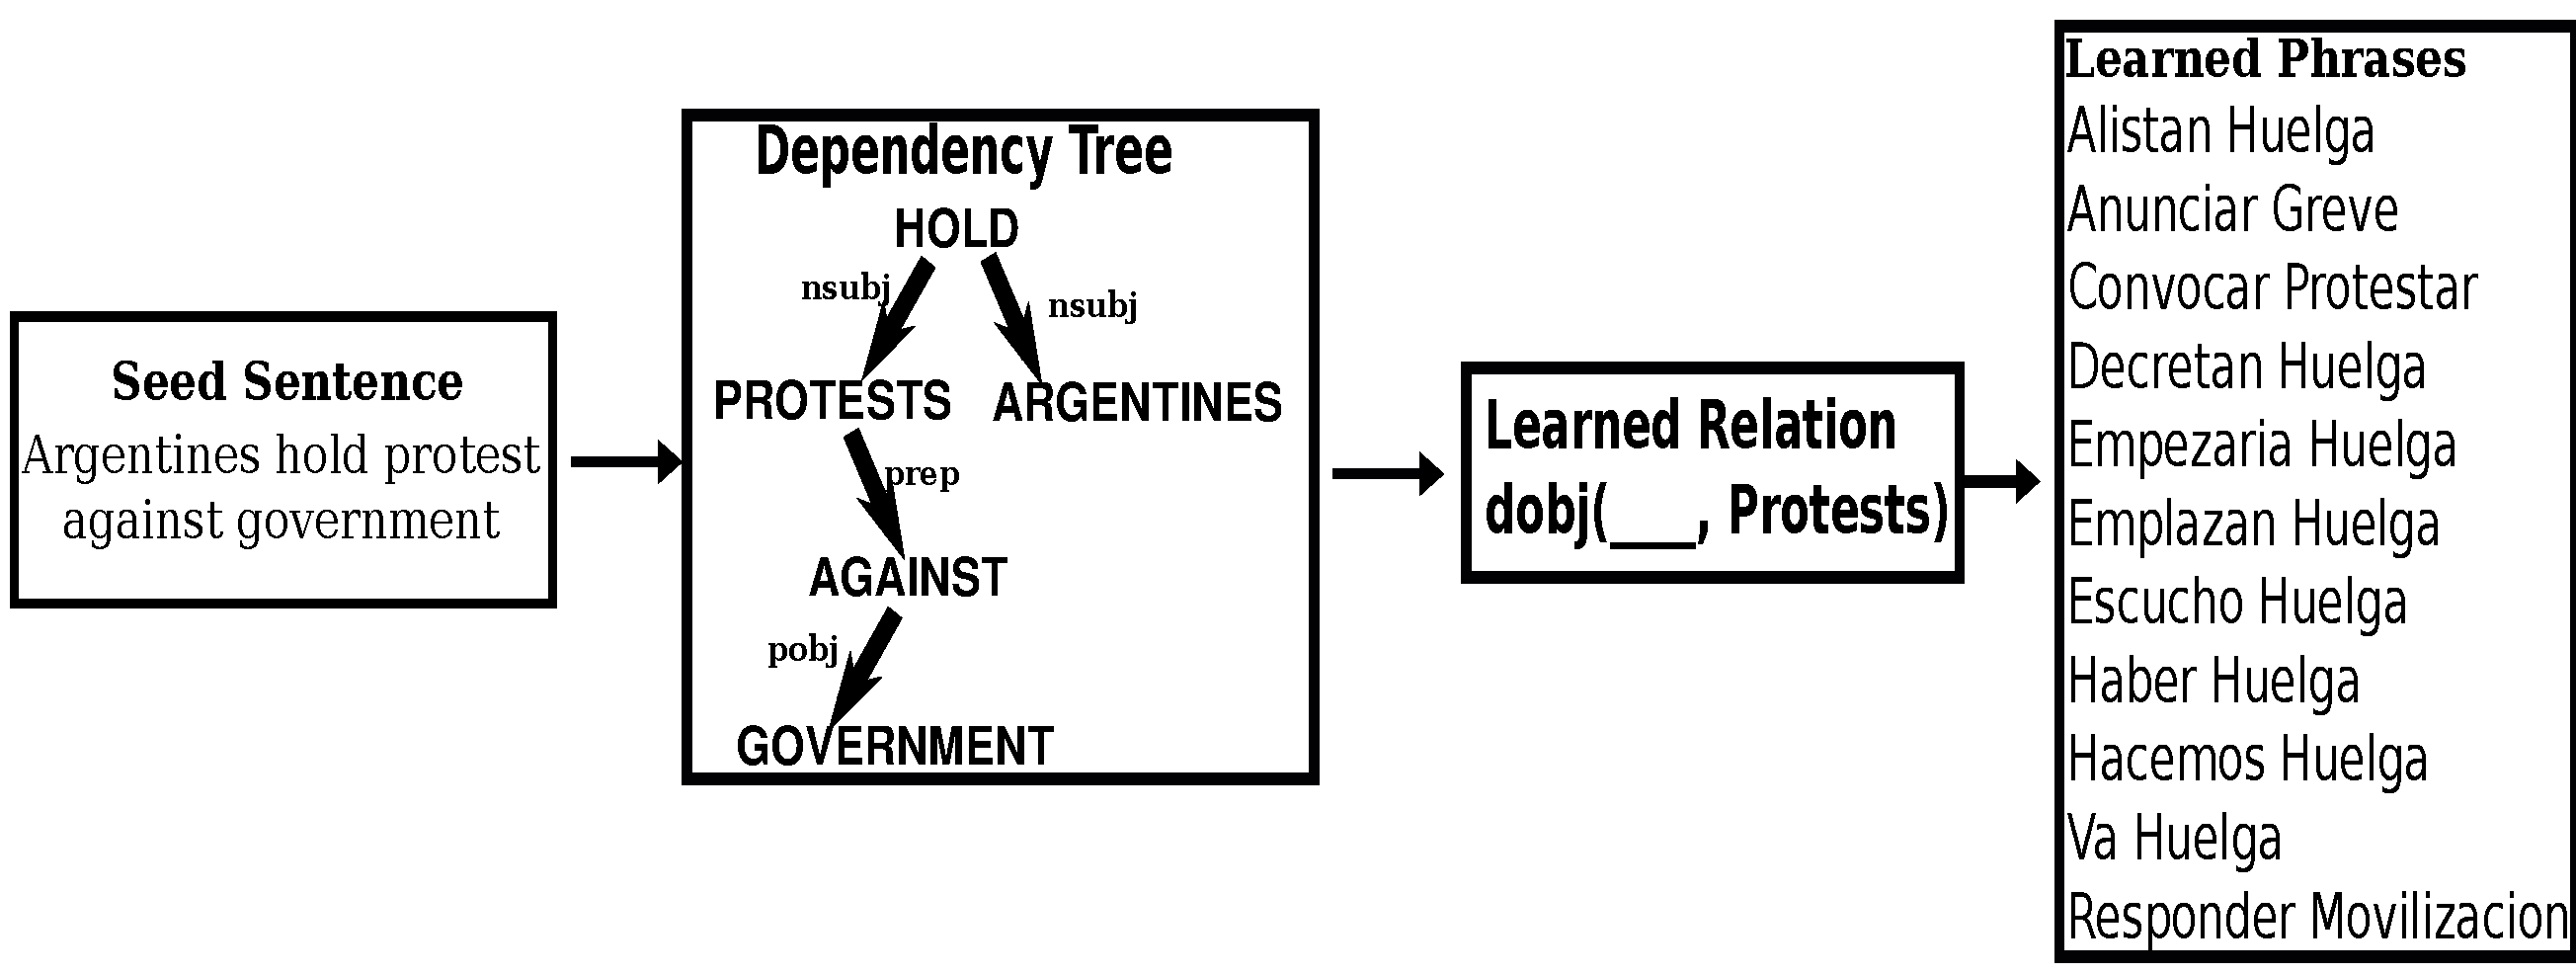
\includegraphics[width=.9\textwidth]{figures/phraseLearning}
\caption{An example of phrase learning for detecting planned protests.}
\label{fig:phraselearning}
\end{figure*}

\subsection{Geocoding}
\label{subsection:geocoding}
After linguistic preprocessing and suitable phrase filtering,
messages are geocoded with a
specification of the geographical focus of the text---specified as a
city, state, country triple---that indicates the locality that the
text is about. We make use of different geocoding methodologies
for Twitter messages, for Facebook Events pages, and for news articles and blogs.
These are described below.

\subsubsection{Twitter and Facebook}
For tweets, the geographic focus of the message is generated by a fairly simple
set of heuristics involving i) the most reliable but least available
source, i.e., the geotag (latitude, longitude) of the tweet itself, ii)
Twitter {\it places} metadata, and iii) if the above are not available,
the text fields contained in the user profile (location, description) as
well as the tweet text itself to find mentions of relevant locations.
Additional toponym disambiguation heuristics are used to identify the
actual referent of the mention.  Similar methods are used to geocode
event data extracted from Facebook event pages.  

\subsubsection{News and Blogs}
For longer articles such as news articles, the geographic focus of the message
is identified using much more complex methods to extract the protest
location from news articles. We use PSL to build a probabilistic model
that infers the intended location of a protest by weighing evidence
coming from entities extracted by the RLP preprocessor and information in the World
Gazetteer. 

The primary rules in the model encode the effect that RLP extracted
location strings that match to gazetteer aliases are indicators of the
article's location, whether they be country, state, or city aliases.
Each of these implications is conjuncted with a prior for ambiguous,
overloaded aliases that is proportional to the population of the
gazetteer location. For example, if the string ``Los Angeles'' appears
in the article, it could refer to either Los Angeles, California, or Los
\'{A}ngeles in Argentina or Chile. Given no other information, our model
would infer a higher truth value for the article referring to Los
Angeles, California, because it has a much higher population than the
other options. 
\begin{equation*}
  \begin{array}{rcl}
  \textsc{Entity}(L, \textrm{location}) \softand \textsc{RefersTo}(L,\textrm{locID}) & \rightarrow & \textsc{PSLLocation}(\textrm{Article}, \textrm{locID})\\
  \\
  \textsc{Entity}(C, \textrm{location}) \softand \textsc{IsCountry}(C)               & \rightarrow & \textsc{ArticleCountry}(\textrm{Article}, C)\\
  \\
  \textsc{Entity}(S, \textrm{location}) \softand \textsc{IsState}(S)                 & \rightarrow & \textsc{ArticleState}(\textrm{Article}, S)\\
  \\
  \end{array}
\end{equation*}

\noindent
(Note that the above are not deterministic rules; e.g., they do not use
the logical conjunction but rather the Lukasiewicz t-norm based
relaxation. Further, these rules do not fire deterministically but are
instead simultaneously solved for satisfying assignments as described in
the section on Probabilistic Soft Logic (PSL).)

The secondary rules, which are given half the weight of the primary
rules, perform the same mapping of extracted strings to gazetteer
aliases, but for extracted persons and organizations. Strings describing
persons and organizations often include location clues (e.g., ``mayor of
Buenos Aires''), but intuition suggests the correlation between the
article's location and these clues may be lower than with location
strings. 
\begin{equation*}
  \begin{array}{rcl}
  \textsc{Entity}(O, \textrm{organization})  \softand  \textsc{RefersTo}(O, \textrm{locID}) & \rightarrow &  \textsc{PSLLocation}(\textrm{Article},\textrm{locID})\\
  \\
  \textsc{Entity}(O, \textrm{organization}) \softand   \textsc{IsCountry}(O)                & \rightarrow &  \textsc{ArticleCountry}(\textrm{Article}, O)\\
  \\
  \textsc{Entity}(O, \textrm{organization}) \softand \textsc{IsState}(O)                    & \rightarrow & \textsc{ArticleState}(\textrm{Article}, O)\\
  \end{array}
\end{equation*}

Finally, the model includes rules and constraints to require consistency
between the different levels of geolocation, making the model place
higher probability on states with its city contained in its state, which
is contained in its country. As a post-processing step, we enforce this
consistency explicitly by using the inferred city and its enclosing
state and country, but adding these rules into the model make the
probabilistic inference prefer consistent predictions, enabling it to
combine evidence at all levels.
\begin{equation*}
  \begin{array}{rcl}
  \textsc{PSLLocation}(\textrm{Article}, \textrm{locID}) \softand \textsc{Country}(\textrm{locID}, C) & \rightarrow & \textsc{ArticleCountry}(\textrm{Article}, C) \\
  \\
  \textsc{PSLLocation}(\textrm{Article}, \textrm{locID}) \softand \textsc{Admin1}(\textrm{locID}, S)  & \rightarrow & \textsc{ArticleState}(\textrm{Article}, S) \\
  \end{array}
\end{equation*}

As an example of how PSL aids in location identification,
the protest from Fig.~\ref{pp_example} is revisited in
Fig.~\ref{fig:psl_example}, which illustrates
the evidence that the PSL model gathers from the news article and the
inferred locations.

\begin{figure*}
  \centering
%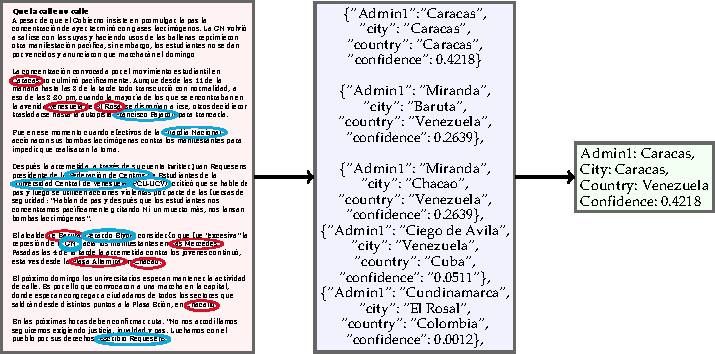
\includegraphics[width=\textwidth]{figures/psl_pipeline_tikz}
\caption{An example of location inference using PSL. Red circles
   denote named entities identified as locations and blue denotes other
   types of entities. The article describes students planning a march on
   Sunday.  It identifies multiple locations, e.g., Chacao, El Roso, and
   the Francisco Fajardo highway where protests have been happening.
   There is also a reference to a quote by the mayor of Baruto.
   Mentions of such multiple locations are resolved using our PSL
   program to the intended location, here Caracas.}
\label{fig:psl_example}
\end{figure*}
%######################EXPERIMENTS#####################################
We evaluate our planned protest detection system for Latin America using
metrics similar to those described in Ramakrishnan et
al.~\shortcite{emberskdd}.  Given a set of alerts issued by the system
and the GSR comprising actual protest incidents, we aim to identify a
correspondence between the two sets via a bipartite matching.  An alert
can be matched to a GSR event only if i) they are both issued for the
same country, ii) the alert's predicted location and the event's
reported location are within 300km of each other (the distance offset),
and iii) the forecast event date is within a given interval of the true
event date (the date offset).  Once these inclusion criteria apply, the
quality score (QS) of the match is defined as a combination of the
location score (LS) and date score (DS):
\small
\begin{equation}
    \operatorname{QS}= (LS + DS)*2
\end{equation}
\normalsize
\noindent
where
\small
\begin{equation}
    \operatorname{LS}=1 - \frac{\min(\textrm{distance offset}, 300)}{300}
\end{equation}
and 
\begin{equation}
    \operatorname{DS}=1 - \frac{\min(\textrm{date offset}, \operatorname{INTERVAL})}{\operatorname{INTERVAL}}
\end{equation}
\normalsize
Here, we explore $\operatorname{INTERVAL}$ values from \textsc{0} to
\textsc{7}.  If
an alert (conversely, GSR event) cannot be matched to any GSR event
(alert, respectively), these unmatched alerts (and events) will
negatively impact the precision (and recall) of the system. The lead
time, for a matched alert-event pair, is calculated as the difference
between the date on which the forecast was made and the date on which
the event was reported (this should not be confused with the date score,
which is the difference between the predicted event date and the actual
event date). Lead time concerns itself with reporting and forecasting,
whereas the date score is concerned with quality or accuracy.

We conduct a series of experiments to evaluate the performance of our
system.\\

\noindent
{\bf How does the distribution of protests detected by the system
compare with the actual distribution of protests in the GSR?}
Fig.~\ref{fig:distribution} reveals pie charts of both distributions. As
shown, Mexico, Brazil, and Venezuela experience the lion's share of
protests in our region of interest, and the protests detected also match
these modes although not the specific percentages. Smaller countries
like Ecuador, El Salvador, and Uruguay do experience protests but which
are not as prominently detected as those for other countries; we
attribute this to their smaller social media footprint (relative to
countries like Brazil and Venezuela).\\
\begin{figure*}
%\centering
\begin{subfigure}{0.4\columnwidth}
  \raggedleft
  %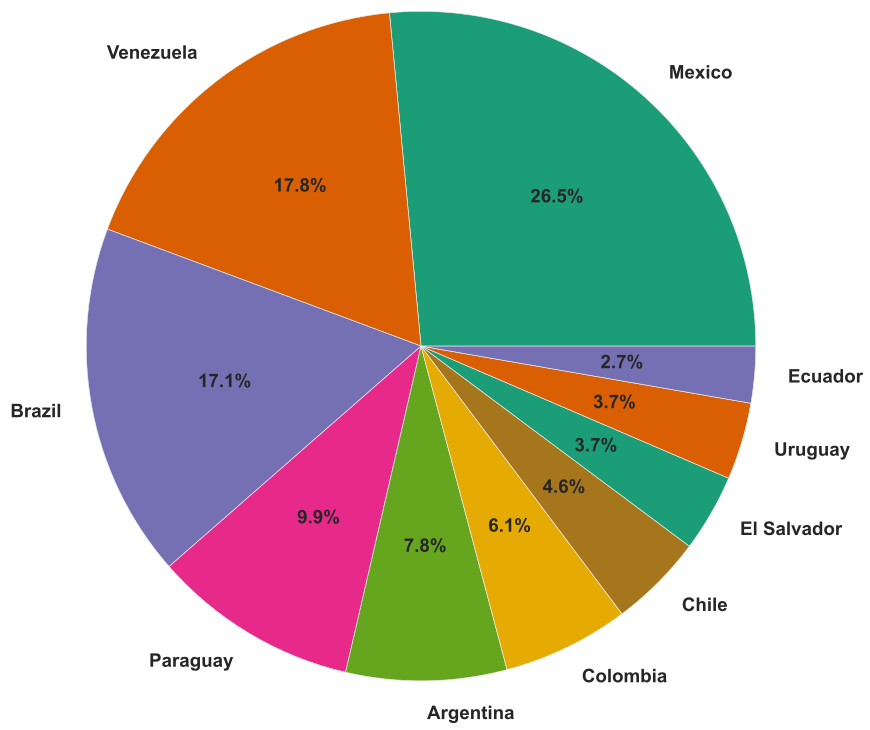
\includegraphics[height=.2\textheight]{gsr_distribution} 
  \caption{\scriptsize GSR distribution from 2012-11 to 2014-03.}
  \label{fig:gsrdistribution}
\end{subfigure}\hspace{3.2em}%
\begin{subfigure}{.4\columnwidth}
  \raggedright
  %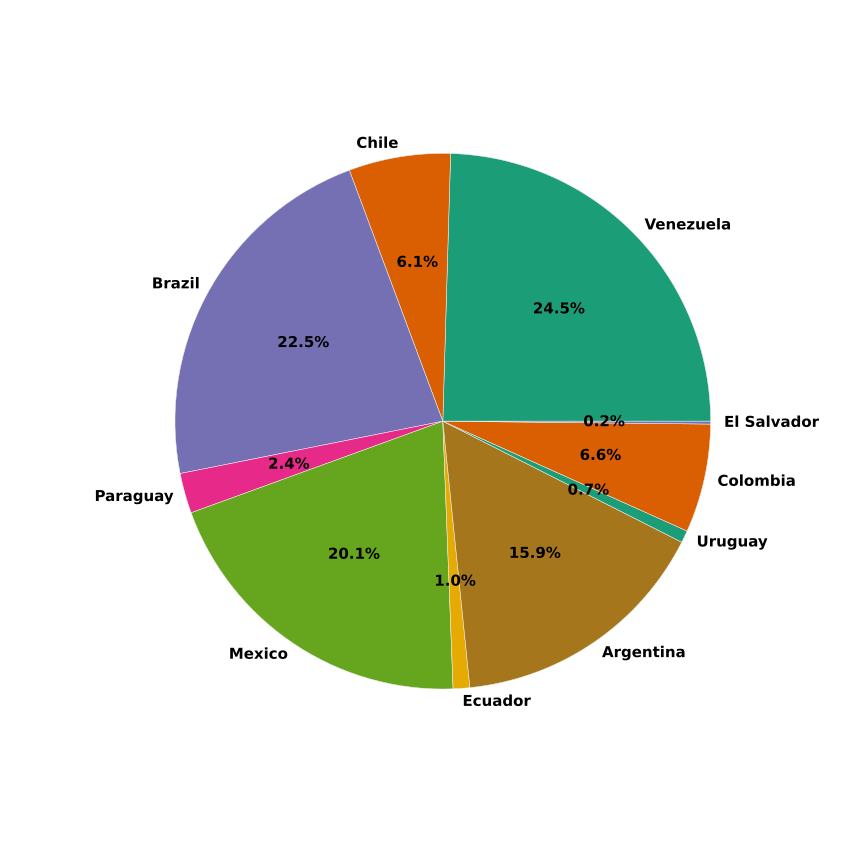
\includegraphics[height=.2\textheight]{pp_dist}
  \caption{\scriptsize Alerts distribution from 2012-11 to 2014-03.}
  \label{fig:ppdistribution}
\end{subfigure}
\caption{Distribution of alerts and GSR events across the Latin American countries studied in this paper.}
\label{fig:distribution}
\end{figure*}

\newpage
\begin{table}
    \scriptsize
    \centering
    \caption{\label{tb:sourcewisecomparison} 
    \small Country-wise breakdown of forecasting performance for different data sources.
QS=Quality Score; Pr=Precision; Rec=Recall; LT=Lead Time.
AR=Argentina; BR=Brazil; CL=Chile; CO=Colombia; EC=Ecuador;SV=El Salvador; 
MX=Mexico; PY=Paraguay; UY=Uruguay; VE=Venezuela. A $-$
indicates that the source did not produce any warnings for that country
in the studied period.}
\begin{tabularx}{.9\textwidth}{*{17}{X}} %{@{}rrrrrrrrrrrrrrrrr@{}}
        \toprule
        & \multicolumn{4}{c}{News/Blogs} & \multicolumn{4}{c}{Twitter} & \multicolumn{4}{c}{Facebook} & \multicolumn{4}{c}{Combined}\\
        \midrule
         & QS & Pr. & Rec. &LT & QS & Pr. & Rec. & LT & QS & Pr. & Rec. & LT & QS & Pr. & Rec. & LT\\
        \midrule
        AR &3.14&0.32&0.69&3.94&3.52&{\bf0.78}&0.14&3.14&{\bf3.70}&0.50&0.04&3.00&3.02&0.36&{\bf0.80}&{\bf4.50}\\
        BR &3.14&0.48&0.54&{\bf5.85}&-&-&-&-&{\bf3.62}&{\bf0.76}&0.18&2.46&3.28&0.49&{\bf0.65}&5.15\\
        CL &3.06&0.91&0.67&5.40&{\bf3.52}&{\bf1.00}&0.23&4.29&-&-&-&-&3.16&0.83&{\bf0.80}&{\bf5.92}\\
        CO &2.74&0.90&0.56&{\bf7.44}&3.30&{\bf1.00}&0.15&2.43&{\bf4.00}&{\bf1.00}&0.02&2.00&2.88&0.84&{\bf0.65}&6.47\\
        EC &-&-&-&-&{\bf2.32}&{\bf1.00}&{\bf0.06}&{\bf17.00}&-&-&-&-&{\bf2.32}&{\bf0.50}&{\bf0.06}&{\bf17.00}\\
        MX &2.96&0.88&0.25&{\bf3.69}&3.14&{\bf1.00}&0.02&1.43&{\bf3.72}&0.67&0.01&2.00&3.00&0.87&{\bf0.27}&3.51\\
        SV &{\bf3.22}&{\bf1.00}&{\bf0.03}&{\bf1.00}&-&-&-&-&-&-&-&-&{\bf3.22}&{\bf1.00}&{\bf0.03}&{\bf1.00}\\
        PY &3.38&{\bf1.00}&{\bf0.16}&9.11&3.84&{\bf1.00}&0.04&{\bf11.40}&3.96&{\bf1.00}&0.01&2.00&3.60&0.96&{\bf0.20}&9.35\\
        UY &{\bf3.24}&{\bf1.00}&{\bf0.29}&{\bf2.40}&-&-&-&-&-&-&-&-&3.24&{\bf1.00}&{\bf0.29}&3.24\\
        VE &{\bf3.80}&{\bf1.00}&0.36&{\bf3.27}&3.68&0.97&0.33&2.39&-&-&-&-&3.64&0.99&{\bf0.69}&2.88\\
        ALL &3.34&0.69&0.35&{\bf4.57}&3.62&{\bf0.97}&0.15&2.82&3.66&0.74&0.03&2.44&3.36&0.73&{\bf0.51}&4.08\\
        \bottomrule
    \end{tabularx}
\end{table}
\newpage
~
\newpage

\newpage
\begin{table*} %[tb!]
  \footnotesize
\centering
\caption{\small Comparing the location and date scores of different sources in specific countries.
AR=Argentina; BR=Brazil; CL=Chile; CO=Colombia; EC=Ecuador;SV=El
Salvador; MX=Mexico; PY=Paraguay; UY=Uruguay; VE=Venezuela. A $-$
indicates that the source did not produce any warnings for that country
in the studied period.} \label{tb:modelwisecomparison}
%\begin{tabular}{@{}ccccccccccccccccc{}@}
\begin{tabularx}{.9\textwidth}{p{1.7cm}*{16}{X}}
\toprule
Source& & AR & BR & CL & CO & EC & SV & MX & PY & UY & VE & All\\
\midrule
\multirow{2}{*}{News/Blogs} &LS &0.82&0.76&0.75&0.60&-&{\bf0.75}&0.66&0.79&{\bf0.79}&{\bf0.95}&0.81\\
                            &DS&0.75&0.81&0.78&0.77&-&{\bf0.86}&0.82&0.90&{\bf0.83}&{\bf0.95}&0.86\\
\midrule
\multirow{2}{*}{Facebook} &LS &{\bf1.0}&{\bf0.92}&-&{\bf1.00}&-&-&{\bf0.86}&{\bf0.98}&-&-&{\bf0.93}\\
                          &DS&0.85&{\bf0.89}&-&{\bf1.00}&-&-&{\bf1.00}&{\bf1.00}&-&-&0.90\\
\midrule
\multirow{2}{*}{Twitter} &LS &0.88&-&{\bf0.84}&0.81&{\bf0.45}&-&0.71&{\bf0.98}&-&0.91&0.89\\
                         &DS&{\bf0.88}&-&{\bf0.92}&0.84&{\bf0.71}&-&0.86&0.94&-&0.93&{\bf0.92}\\
\bottomrule
\end{tabularx}
\end{table*}
\newpage
~
\newpage

\noindent
{\bf Are there country-specific selective superiorities for the
different data sources considered here?}
Table~\ref{tb:sourcewisecomparison} presents a breakdown of performance,
country-wise and source-wise, of our approach for a particular month,
viz. March 2014.  It is clear that the multiple data sources are
necessary to achieve a high recall and that by and large these sources
are providing mutually exclusive alerts. (Note also that some data
sources do not produce alerts for specific countries.) Between Twitter
and Facebook, the former is a better source of alerts for countries like
Chile and the latter is a better source for Argentina, Brazil, Colombia,
and Mexico.  News and blogs achieve higher recall than social media
sources indicating that most plans for protests are announced in
established media. They are also higher quality sources for alerts in
countries like El Salvador, Paraguay, and Uruguay.  Finally, note that
news and blogs offer a much higher lead time (4.57 days) as compared to
that for Facebook (2.44 days) or for Twitter (2.82 days). The quality
scores are further broken down in Table~\ref{tb:modelwisecomparison}
into their date and location components.

A longitudinal perspective on quality scores is given in
Fig.~\ref{fig:monthlyqs}. Note that in general Twitter tends to have a
higher quality score as multiple re-tweets of future event mentions is a
direct indicator of the popularity of an event as well as the intent of
people to join an event.  In contrast, mentions of future events in news
do not directly shed any insight into popularity or people's support for
the event's causes.\\

\noindent
{\bf How did our system fare in detecting key country-wide protests?}

The recent Venezuelan protests against President Nicolas Maduro and the
Brazilian protests during June 2013 against bus fare hikes were two
significant protests during our period of evaluation.
Fig.~\ref{fig:venezuela_feb} and Fig.~\ref{fig:brazil_june} describe our
performance under these two situations illustrating the count of
protests detected against the GSR. Notice that our system was able to
identify the Venezuelan protests much better than the Brazilian
protests. This is because there was a significant amount of spontaneity
to the Brazilian protests; they arose as discontent about bus fare
increases but later morphed into a broader set of protests against
government and most of these subsequent protests were not planned.\\

\noindent
{\bf What is the trade-off between lead time and quality?}

Fig.~\ref{fig:leadTimeVsQS} shows that the QS of the planned protest
model decreases (as expected) with lead time, initially, but later rises
again. The higher quality scores toward the right of
Fig.~\ref{fig:leadTimeVsQS} are primarily due to Facebook event pages.\\

\noindent {\bf How does the method perform under stringent matching
criteria?} Fig.~\ref{fig:matchinginterval} shows the performance of the
model when the matching window is varied from 7 to 1 in steps.  We can
see that the performance degrades quite gracefully even under the strict
matching interval of a 1-day difference.\\

\noindent {\bf What is the distribution of quality scores?} The clear
mode toward the right side of the Fig.~\ref{fig:doubleHump} signifies
that a majority of the planned protest alerts are of high quality.
Further, the quality score distribution is unimodal suggesting that the
careful reasoning of locations and date normalization are crucial to
achieving high quality.

\begin{figure*}
\begin{subfigure}{0.33\columnwidth}
    \centering
  %
\includegraphics[width=0.85\columnwidth]{monthlyqs}
  \caption{\scriptsize Quality Score over the months}
  \label{fig:monthlyqs}
\end{subfigure}%\hspace{.5pt}
\begin{subfigure}{0.33\columnwidth}
    \centering
  %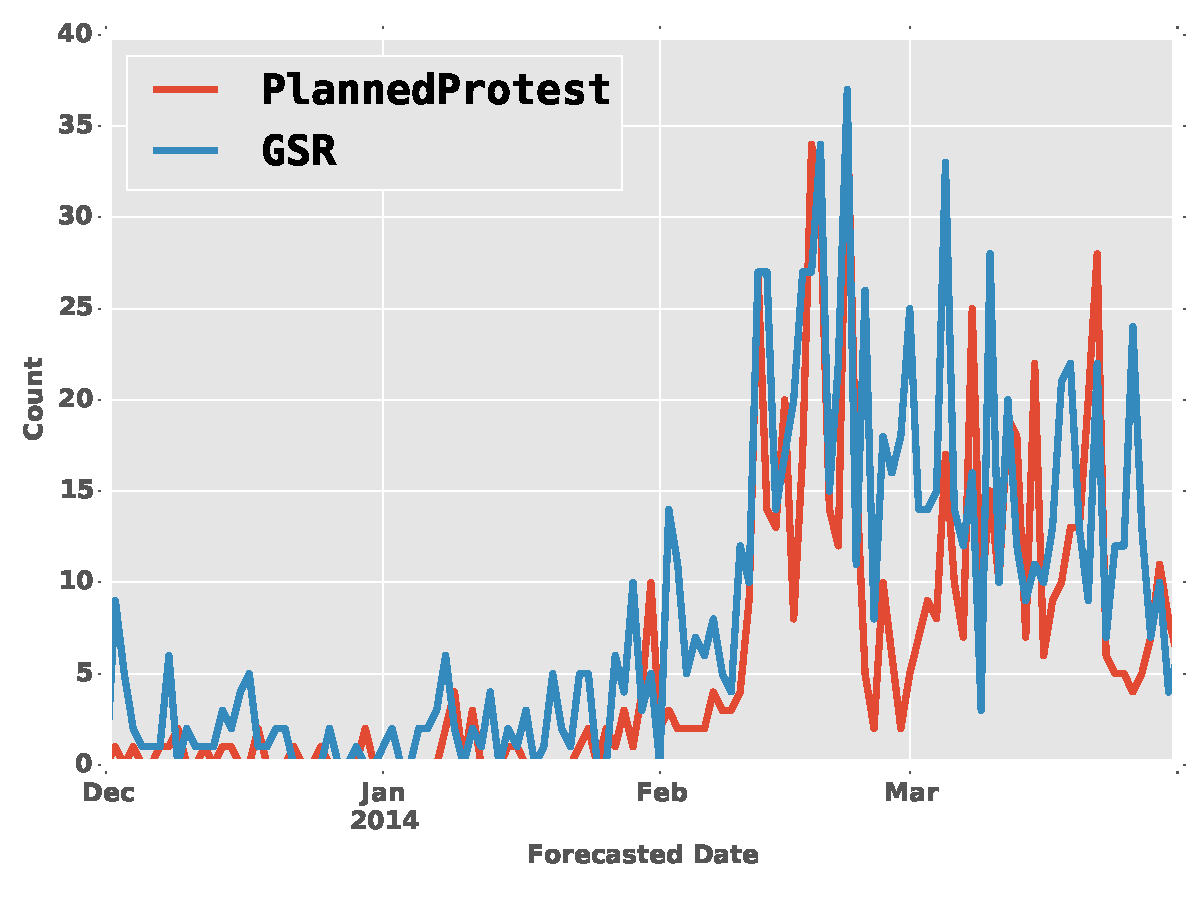
\includegraphics[width=0.85\columnwidth]{venezuela_new}
  \caption{\scriptsize Venezuelan Protests}
  \label{fig:venezuela_feb}
\end{subfigure}%\hspace{.5pt}
\begin{subfigure}{0.33\columnwidth}
    \centering
  %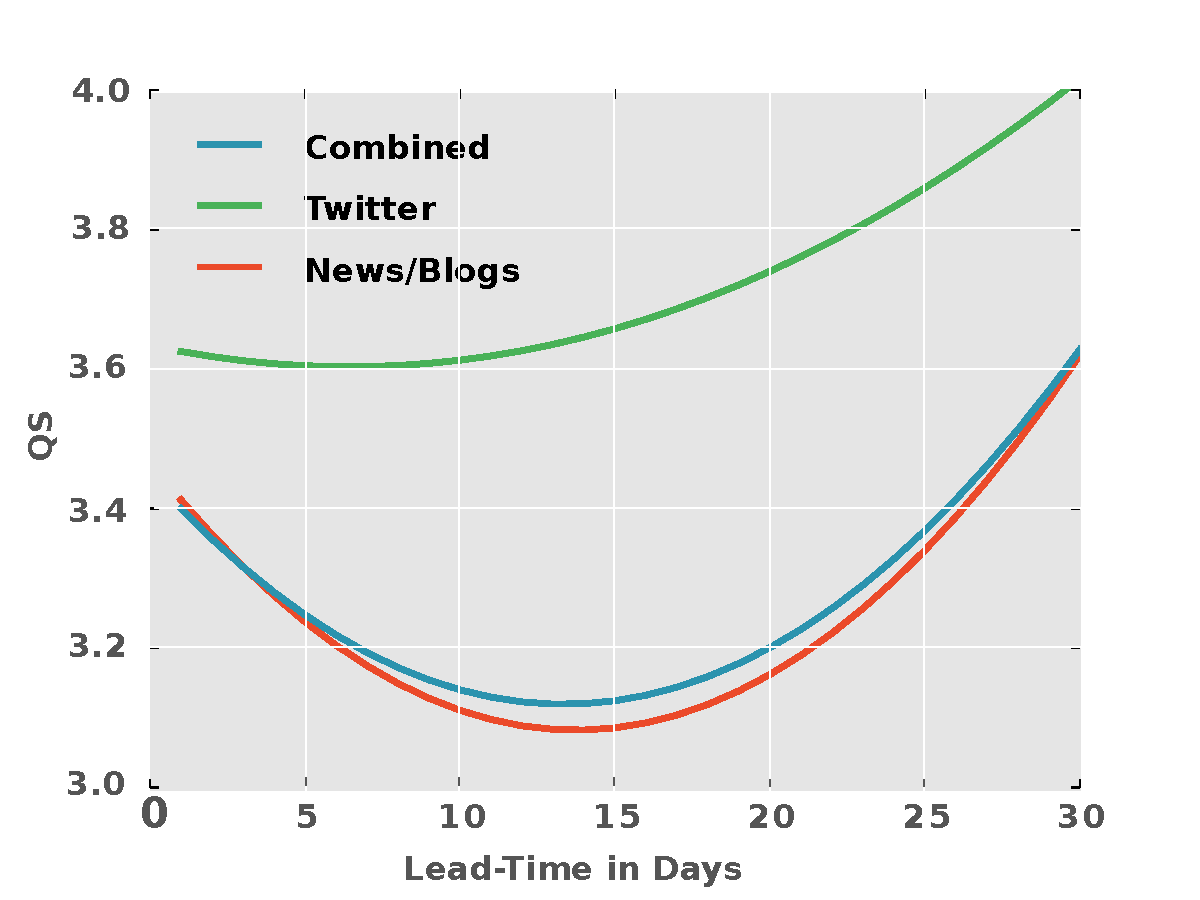
\includegraphics[width=0.85\columnwidth]{leadTimeVsQS}
  \caption{\scriptsize Lead-Time vs Quality Score}
  \label{fig:leadTimeVsQS}
\end{subfigure}

\begin{subfigure}{0.33\columnwidth}
    \centering
  %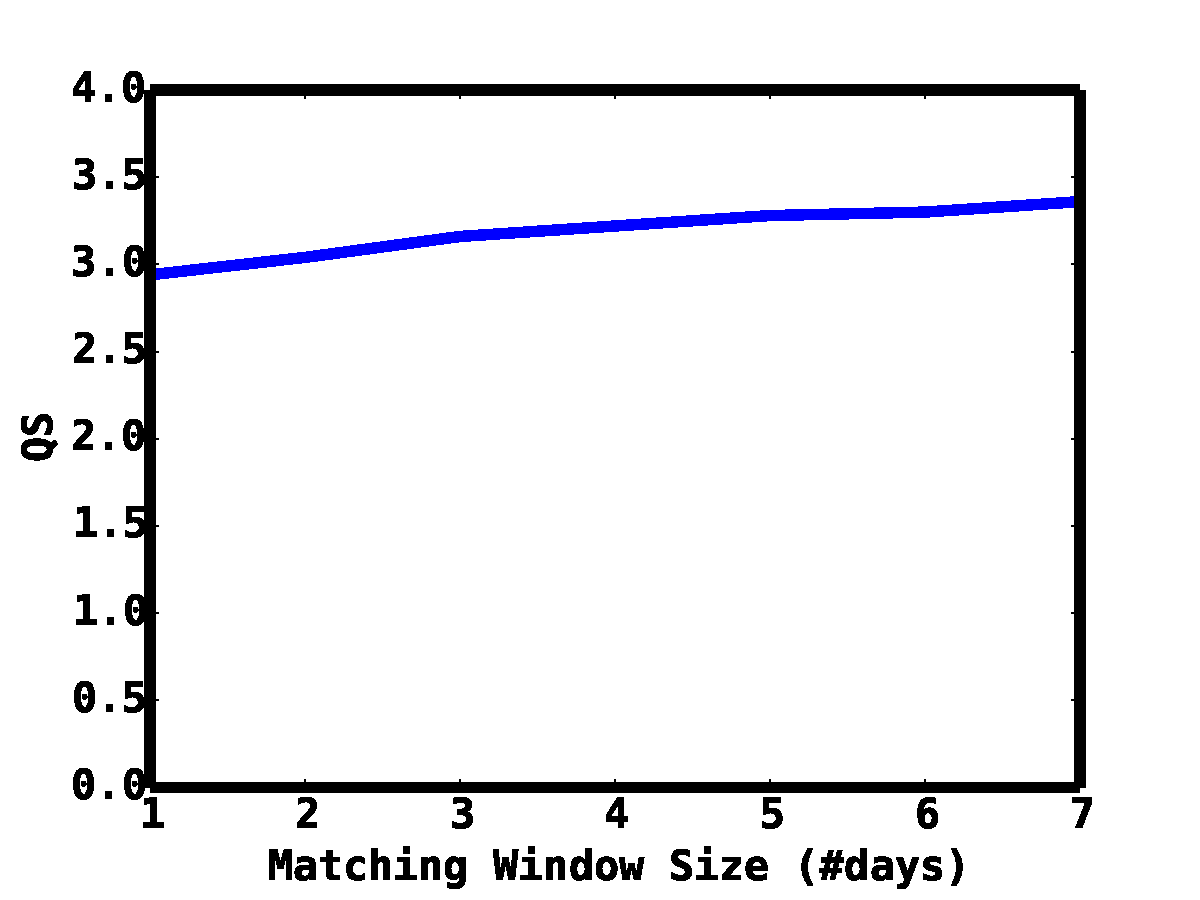
\includegraphics[width=0.85\columnwidth]{matchingwindow}
  \caption{\scriptsize QS vs Matching Interval Trade-Off}
  \label{fig:matchinginterval}
\end{subfigure}%\hspace{.5pt}
\begin{subfigure}{0.33\columnwidth}
    \centering
  %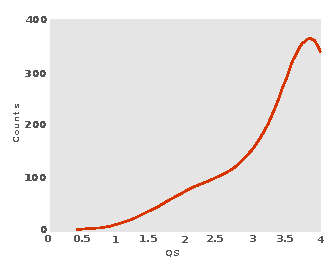
\includegraphics[width=0.85\columnwidth]{doubleHump_new3}
  \caption{\scriptsize Quality Score Distribution}
  \label{fig:doubleHump}
\end{subfigure}%\hspace{.5pt}
\begin{subfigure}{0.33\columnwidth}
    \centering
  %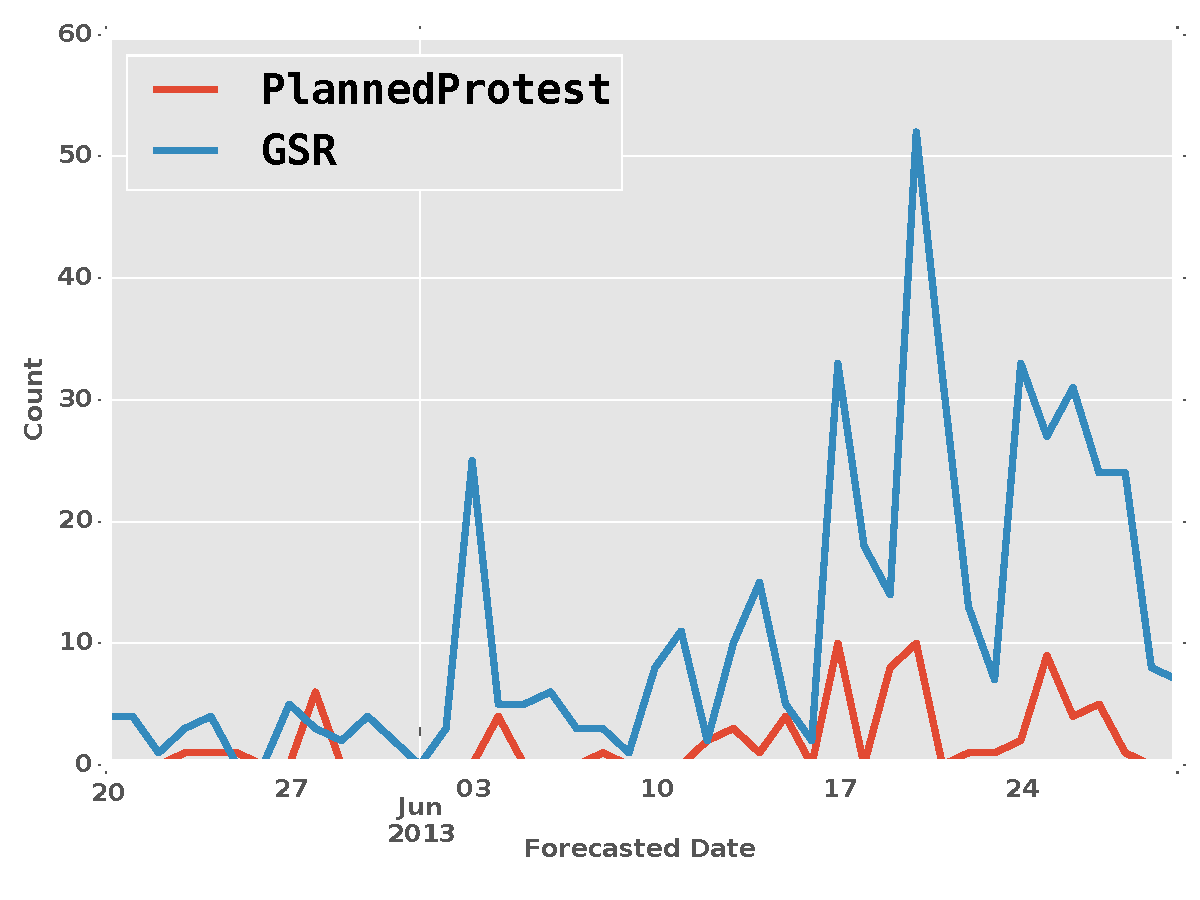
\includegraphics[width=0.85\columnwidth]{brazil_june_new}
  \caption{\scriptsize Brazilian Spring}
  \label{fig:brazil_june}
\end{subfigure}
\caption{Evaluation of planned protest forecasting system}
\end{figure*}%###############Development and Maintenance################


\section{Development and Maintenance}
The core algorithms behind the
planned protest detector were implemented in Python. The PSL geocoder was
implemented in Java. Among the external libraries utilized the Basis Rosette Linguistic Platform is the key
library. The development process took 3 months (June
2012 to Aug 2012) and was
primarily led by the first author with contributions from the other authors.
After two months of testing (Sep 2012 and Oct 2012), the system was deployed
in Nov 2012 on the commercial AWS (Amazon
Web Services) cloud infrastructure in a cluster configuration. 
More details about the EMBERS 
system architecture can be found in
Doyle et al.~\shortcite{DBLP:conf/bigdataconf/DoyleKSAZLMZLBKFR14}. Alerts
generated by the system are automatically emailed to MITRE (for evaluation)
as well as to analysts who are subject matter experts in Latin America.

Since there is not an explicit training
phase, the system has required minimal re-engineering over time. Key changes
made to the system over time was to increase the sources used for data ingest
and supporting the inclusion of additional phrases. Agile software
engineering methods were used for project management. We estimate the
effort to maintain the system as 0.25 persons (software engineer) per year
which entails keeping data sources current, ensuring that
the phrase list continues to stay relevant, and performing periodic 
checks and evaluations of the sytem.

\section{Discussion}
We have described an approach to forecasting protests by detecting
mentions of future events in news and social media. The twin issues
of i) resolving the date and ii) resolving the location have been
addressed satisfactorily to realize an effective protest forecasting
system. As different forms of communication media gain usage, systems
like ours will be crucial to understanding the concerns of citizenry.

Our future work is aimed at three aspects. First, to address situations
such as nationwide protests and systems of protests, we must generalize
our system from generating protests at a single article level to
digesting groups of articles. Doing so would require more sophisticated
probabilistic reasoning, which we believe can be done using PSL.
Second, we would like to generalize our
approach that currently does detection of overt plans for protest to
not-so-explicitly stated expressions of discontent.  Finally, we plan to
consider other population-level events of interest than just civil
unrest, e.g., domestic political crises, and design detectors to
recognize the imminence of such events.

\section*{Acknowledgments}
Supported by the Intelligence Advanced Research Projects Activity (IARPA) via
DoI/NBC contract number D12PC000337, the US Government is authorized to
reproduce and distribute reprints of this work for Governmental purposes
notwithstanding any copyright annotation thereon.  Disclaimer: The views and
conclusions contained herein are those of the authors and should not be
interpreted as necessarily representing the official policies or endorsements,
either expressed or implied, of IARPA, DoI/NBC, or the US Government.

%\bibliographystyle{aaai}
%\bibliography{references}
\begin{thebibliography}{}

\bibitem[\protect\citeauthoryear{Bach \bgroup et al\mbox.\egroup
  }{2013}]{bach:uai13}
Bach, S.~H.; Huang, B.; London, B.; and Getoor, L.
\newblock 2013.
\newblock Hinge-loss {M}arkov {R}andom {F}ields: {C}onvex {I}nference for
  {S}tructured {P}rediction.
\newblock In {\em Uncertainty in Artificial Intelligence}.

\bibitem[\protect\citeauthoryear{Baeza-Yates}{2005}]{baeza2005searching}
Baeza-Yates, R.
\newblock 2005.
\newblock Searching the {F}uture.
\newblock In {\em SIGIR Workshop on Mathematical/Formal Methods in Information
  Retrieval}.

\bibitem[\protect\citeauthoryear{Banko \bgroup et al\mbox.\egroup
  }{2007}]{Banko07openinformation}
Banko, M.; Cafarella, M.~J.; Soderland, S.; Broadhead, M.; and Etzioni, O.
\newblock 2007.
\newblock Open {I}nformation {E}xtraction from the {W}eb.
\newblock In {\em International Joint Conferences on Artificial Intelligence},
  IJCAI.

\bibitem[\protect\citeauthoryear{Chambers and
  Jurafsky}{2011}]{Chambers:2011:TIE}
Chambers, N., and Jurafsky, D.
\newblock 2011.
\newblock Template-based {I}nformation {E}xtraction {W}ithout the {T}emplates.
\newblock In {\em Proceedings of the 49th Annual Meeting of the Association for
  Computational Linguistics: Human Language Technologies}, HLT.

\bibitem[\protect\citeauthoryear{Compton \bgroup et al\mbox.\egroup
  }{2013}]{compton2013detecting}
Compton, R.; Lee, C.; Lu, T.-C.; De~Silva, L.; and Macy, M.
\newblock 2013.
\newblock {D}etecting {F}uture {S}ocial {U}nrest in {U}nprocessed {T}witter
  {D}ata:“{E}merging {P}henomena and {B}ig data”.
\newblock In {\em IEEE International Conference on Intelligence and Security
  Informatics}, ISI.

\bibitem[\protect\citeauthoryear{Doyle \bgroup et al\mbox.\egroup
  }{2014}]{DBLP:conf/bigdataconf/DoyleKSAZLMZLBKFR14}
Doyle, A.; Katz, G.; Summers, K.~M.; Ackermann, C.; Zavorin, I.; Lim, Z.;
  Muthiah, S.; Zhao, L.; Lu, C.; Butler, P.; Khandpur, R.~P.; Fayed, Y.; and
  Ramakrishnan, N.
\newblock 2014.
\newblock The {EMBERS} {A}rchitecture for {S}treaming {P}redictive {A}nalytics.
\newblock In {\em {IEEE} International Conference on Big Data}.

\bibitem[\protect\citeauthoryear{Gabrilovich, Dumais, and
  Horvitz}{2004}]{Gabrilovich:2004:NPP}
Gabrilovich, E.; Dumais, S.; and Horvitz, E.
\newblock 2004.
\newblock Newsjunkie: {P}roviding {P}ersonalized {N}ewsfeeds via {A}nalysis of
  {I}nformation {N}ovelty.
\newblock In {\em Proceedings of the International Conference on World Wide
  Web}, WWW.

\bibitem[\protect\citeauthoryear{Hurriyetoglu, Kunneman, and van~den
  Bosch}{2013}]{bosch2013estm}
Hurriyetoglu, A.~H.; Kunneman, F.; and van~den Bosch, A.
\newblock 2013.
\newblock Estimating the {T}ime between {T}witter {M}essages and {F}uture
  {E}vents.
\newblock In {\em Proceedings of the Dutch-Belgian Workshop on Information
  Retrieval}, DIR.

\bibitem[\protect\citeauthoryear{Jatowt and Au~Yeung}{2011}]{Jatowt:2011:ECE}
Jatowt, A., and Au~Yeung, C.~m.
\newblock 2011.
\newblock Extracting {C}ollective {E}xpectations {A}bout the {F}uture from
  {L}arge {T}ext {C}ollections.
\newblock In {\em Proceedings of the 20th ACM International Conference on
  Information and Knowledge Management}, CIKM.

\bibitem[\protect\citeauthoryear{Kallus}{2014}]{nathankallus}
Kallus, N.
\newblock 2014.
\newblock {P}redicting {C}rowd {B}ehavior with {B}ig {P}ublic {D}ata.
\newblock In {\em Proceedings of the 23rd international conference on World
  wide web}, WWW.

\bibitem[\protect\citeauthoryear{Kawai \bgroup et al\mbox.\egroup
  }{2010}]{Kawai:2010:CSE}
Kawai, H.; Jatowt, A.; Tanaka, K.; Kunieda, K.; and Yamada, K.
\newblock 2010.
\newblock {ChronoSeeker: Search Engine for Future and Past Events}.
\newblock In {\em Proceedings of the International Conference on Uniquitous
  Information Management and Communication}, ICUIMC.

\bibitem[\protect\citeauthoryear{Kimmig \bgroup et al\mbox.\egroup
  }{2012}]{kimmig2012short}
Kimmig, A.; Bach, S.; Broecheler, M.; Huang, B.; and Getoor, L.
\newblock 2012.
\newblock A {S}hort {I}ntroduction to {P}robabilistic {S}oft {L}ogic.
\newblock In {\em Proceedings of the NIPS Workshop on Probabilistic
  Programming: Foundations and Applications}.

\bibitem[\protect\citeauthoryear{Llorens \bgroup et al\mbox.\egroup
  }{2012}]{LlorensDGS12}
Llorens, H.; Derczynski, L.; Gaizauskas, R.~J.; and Saquete, E.
\newblock 2012.
\newblock {{\sc TIMEN}: An Open Temporal Expression Normalisation Resource.}
\newblock In {\em Proceedings of Language Resources and evaluation}, LREC.

\bibitem[\protect\citeauthoryear{Mani and Wilson}{2000}]{tempex}
Mani, I., and Wilson, G.
\newblock 2000.
\newblock {Robust Temporal Processing of News}.
\newblock In {\em Proceedings of the Annual Meeting on Association for
  Computational Linguistics}, ACL.

\bibitem[\protect\citeauthoryear{Padró and Stanilovsky}{2012}]{freeling}
Padró, L., and Stanilovsky, E.
\newblock 2012.
\newblock {F}reeling 3.0: {T}owards {W}ider {M}ultilinguality.
\newblock In {\em Proceedings of the Language Resources and Evaluation
  Conference}, LREC.

\bibitem[\protect\citeauthoryear{Pustejovsky \bgroup et al\mbox.\egroup
  }{2003}]{timeml}
Pustejovsky, J.; Castano, J.~M.; Ingria, R.; Sauri, R.; Gaizauskas, R.~J.;
  Setzer, A.; Katz, G.; and Radev, D.~R.
\newblock 2003.
\newblock {TimeML: Robust Specification of Event and Temporal Expressions in
  Text.}
\newblock {\em New directions in question answering}.

\bibitem[\protect\citeauthoryear{Radinsky and
  Horvitz}{2013}]{Radinsky:2013:MWP}
Radinsky, K., and Horvitz, E.
\newblock 2013.
\newblock {Mining the Web to Predict Future Events}.
\newblock In {\em Proceedings of the Sixth ACM International Conference on Web
  Search and Data Mining}, WSDM.

\bibitem[\protect\citeauthoryear{Ramakrishnan \bgroup et al\mbox.\egroup
  }{2014}]{emberskdd}
Ramakrishnan, N.; Butler, P.; Muthiah, S.; et~al.
\newblock 2014.
\newblock `{B}eating the news' with {E}{M}{B}{E}{R}{S}: {F}orecasting {C}ivil
  {U}nrest using {O}pen {S}ource {I}ndicators.
\newblock In {\em Proceedings of the International Conference on Knowledge
  Discovery and Data Mining, SIGKDD}.

\bibitem[\protect\citeauthoryear{Riloff and Wiebe}{2003}]{riloff2003learning}
Riloff, E., and Wiebe, J.
\newblock 2003.
\newblock {L}earning {E}xtraction {P}atterns for {S}ubjective {E}xpressions.
\newblock In {\em Proceedings of the conference on Empirical methods in natural
  language processing}, EMNLP.

\bibitem[\protect\citeauthoryear{Str{\"o}tgen \bgroup et al\mbox.\egroup
  }{2014}]{strotgen2014time}
Str{\"o}tgen, J.; Armiti, A.; Van~Canh, T.; Zell, J.; and Gertz, M.
\newblock 2014.
\newblock {T}ime for {M}ore {L}anguages: {T}emporal {T}agging of {A}rabic,
  {I}talian, {S}panish, and {V}ietnamese.
\newblock {\em ACM Transactions on Asian Language Information Processing
  (TALIP)}.

\bibitem[\protect\citeauthoryear{Tops, van~den Bosch, and
  Kunneman}{2013}]{tops2013predicting}
Tops, H.; van~den Bosch, A.; and Kunneman, F.
\newblock 2013.
\newblock {P}redicting {T}ime-to-{E}vent from {T}witter {M}essages.
\newblock In {\em Proceedings of the Benelux Conference on Artificial
  Intelligence}, BNAIC.

\bibitem[\protect\citeauthoryear{Truv{\'e}}{2011}]{recordedFuture}
Truv{\'e}, S.
\newblock 2011.
\newblock {Big Data for the Future: Unlocking the Predictive Power of the Web}.
\newblock {\em Recorded Future, Cambridge, MA, Tech. Rep}.

\bibitem[\protect\citeauthoryear{Verhagen \bgroup et al\mbox.\egroup
  }{2009}]{tempeval}
Verhagen, M.; Gaizauskas, R.; Schilder, F.; Hepple, M.; Moszkowicz, J.; and
  Pustejovsky, J.
\newblock 2009.
\newblock {The TempEval Challenge: Identifying Temporal Relations in Text}.
\newblock {\em Language Resources and Evaluation}.

\bibitem[\protect\citeauthoryear{Xu \bgroup et al\mbox.\egroup
  }{2014}]{xu2014civil}
Xu, J.; Lu, T.-C.; Compton, R.; and Allen, D.
\newblock 2014.
\newblock {C}ivil {U}nrest {P}rediction: {A} {T}umblr-{B}ased {E}xploration.
\newblock In {\em Social Computing, Behavioral-Cultural Modeling and
  Prediction}.

\end{thebibliography}
\par
{\bf Sathappan Muthiah} is a Ph.D student in Computer Science at
Virginia Tech. He is a research assistant at the Discovery Analytics
Center.His research interests include spatial and temporal event
detection, text mining and information retrieval. He received his B.Tech
in Information Technology from National Institute of Technology, Bhopal,
India.
\par

{\bf Bert Huang} is an assistant professor in the Department of Computer
Science at Virginia Tech. Bert's research investigates machine
learning, with a focus on topics including structured prediction,
statistical relational learning, and computational social science. He is
an action editor for the Journal of Machine Learning Research, and his
papers have been published at conferences including NIPS, ICML, UAI, and
AISTATS. He earned his Ph.D.~from Columbia University
in 2011, and he was a postdoctoral research associate at the University
of Maryland, College Park.
\par

{\bf Jaime Arredondo} is a Ph.D. candidate in global public health at UC San
Diego. His research centers on developing more sophisticated analytical
skills and research techniques to analyze the effect of policing
practices as a major driver of HIV transmission, particularly in the
U.S.$-$Mexico border region. Arredondo argues the development of
adequate police education programs that can help build tools to increase
occupational safety, and a public health perspective that incorporates
HIV prevention and harm reduction strategies.\par
\par

{\bf David Mares} is a professor of Political Science at UCSD.
He holds the Institute of the Americas Chair for Inter-American Affairs at UCSD.
He is the author or editor of ten books
and his publications have appeared in English, Spanish, French,
Portuguese, Italian and Chinese. His research and teaching interests
include international conflict, Latin American energy politics, the
political economy of drug policy, and civil-military relations.
\par

{\bf Lise Getoor} is a professor in the Computer Science Department at
the University of California, Santa Cruz.   Her research areas include
machine learning, data integration, and reasoning under uncertainty,
with an emphasis on graph and network data. She is a Fellow of the
Association for Artificial Intelligence, recipient of nine best paper
and best student paper awards, and was co-chair for ICML 2011.
\par

{\bf Graham Katz} earned his PhD in Linguistics and Computational Linguistics
from University of Rochester before becoming a professor in the
Department of Linguistics at Georgetown university between 2007 and
2012.   He held the role of Applied Research Manager at CACI Inc. from
2012-2015, when he contributed greatly to the success of the EMBERS
project.
\par

{\bf Naren Ramakrishnan} is the Thomas L. Phillips Professor of Engineering at
Virginia Tech. He directs the Discovery Analytics Center, a university
center pursuing advanced research in data mining and knowledge discovery
with applications to important areas of national interest. Ramakrishnan
is the principal investigator of the ongoing IARPA OSI (Open Source
Indicators) project aimed at forecasting significant societal events
(disease outbreaks, civil unrest, elections) from open source datasets.
He received his PhD in Computer Sciences from Purdue University.

\end{document}




%%%%%%%%%%%%%%%%%%%%%%%%%%%%%%%%%%%%%%%%%%%%


% EXPLANATIONS

% Begin Your Document with This Preamble
% Note that because we don't want any actual figures in this document (just figure captions), there is no graphics package.
% PDFTeX is *required*

\documentclass[letterpaper]{article}
\usepackage{aaai}

% The following commands reduces the size of the text on a page, making the conversion process easier.
\setlength{\textwidth}{5in}
\setlength{\oddsidemargin}{.75in}
\setlength{\evensidemargin}{.75in}

% Palatino, Helvetica, and Courier are needed for the conversion process.
\usepackage{palatino}
\usepackage{helvet}
\usepackage{courier}

% AI Magazine doesn't use footnotes, we use endnotes. This package gathers all the foonotes at the end of the document, before the bibliography. See below for the commands required to actually place the footnotes.
\usepackage{endnotes}
\let\footnote=\endnote 

% Entering math mode for in-line text math creates font errors. Instead of $a$ use {\it a} or \textit{a}. Instead of $a_{1} use {\it a}\textsubscript{1}. Instead of $a^1$ use \{it a}\textsuperscript{1}. Instead of $A_b$ use {\it A}\textsubscript{\it b} and so on. Reserve math mode for Greek letters $\alpha$.

\usepackage{fixltx2e} %This package allows \textsuperscript and \textsubscript commands

% We don't want any unnecessary hyphens
\usepackage[none]{hyphenat}

% We don't want two spaces after a period
\frenchspacing

% We don't want word justification
\raggedright

% We don't want extra lines between paragraphs, but we do want a paragraph indent
\setlength{\parindent}{10pt}

% We don't want ligatures for the conversion process. This package eliminates them. Leave this commented, however, because it also eliminates em and en dashes, which might cause confusion. We'll uncomment it later.
%\usepackage{microtype}
%\DisableLigatures{encoding = *, family = *} %This package will eliminate ligatures. We will uncomment it in the final compile

% If you use URLs, we want them in a text font. This modified version of the url package makes that possible.
\usepackage{url}
\makeatletter
\def\url@leostyle{%
 \@ifundefined{selectfont}{\def\UrlFont{\sf}}{\def\UrlFont{\rmfamily}}}
\makeatother
\urlstyle{leo}


% Add your title and the list of authors before the \begin{document}, but don't put any affiliations! (The author bio information goes at the end of the article)

\title{Put Your Title Here}
\author{Add Author Names Here, Separated By Commas}

% We will add the copyright notice in the final version.
\nocopyright

\begin{document}
\maketitle	

% Add the one column command right after the \maketitle command
\onecolumn

% Add your abstract as the first paragraph -- don't call it ``abstract."

\begin{quote}
Abstract text goes here.
\end{quote}

% Your introduction goes here, but don't include a section title for it.

Add introductory text paragraphs here as usual.

% After your introduction, include your paper as usual

\section{Section Title}

Paper text.

% The LaTeX Source *MUST* be one file. Do NOT use \input!

% Include each figure caption right after the complete paragraph that first mentions the figure. Use the [h] option to ensure that it goes there.

\begin{figure}[h]
% \includegraphics...  Note that we *don't* want to import the actual graphic -- so any include graphics commands should be eliminated.
\caption{Caption Should Be Mixed Case.}
\label{fig:xxx}
\end{figure}

% If you have a display equation, include it as usual
% \[ ... \]

\section{Acknowledgements}
If you have acknowledgements, put them at the end of your text

% End notes should go right after the acknowledgements (if any) or concluding paragraph, and right before the bibliography. If you *don't* have any notes in your article, these lines should be commented out:

\begingroup
\parindent 0pt
\parskip 2ex
\def\enotesize{\normalsize}
\theendnotes
\endgroup

% Once you've run bibtext, cut and paste the bbl file into your final source
\bibliographystyle{aaai}
\begin{thebibliography}{}
% Include the bbl file in the final LaTeX Source file
\end{thebibliography}

\end{document}


